
            \begin{figure}
                \centering
                \begin{tikzpicture}
                    \pgfplotsset{%
                        width=1\textwidth,
                        height=0.5\textheight
                    }
                    \begin{axis}[
                        xlabel={Start temperature},
                        ylabel={Average dynamic energy (watt)},
                    ]
                    
                        \addplot [mark=none, red, thick]  coordinates {
                        (35, 0.10674460142645986)(45, 0.1120709285337847)(50, 0.11366270243441509)(55, 0.11976660990043786)(60, 0.12163525241817351)
                        };
                        \addlegendentry{Surface4Pro - IntelPowerGadget}
                        
                        \addplot [mark=none, red, dotted]  coordinates {
                        (35, 0.08686375948005347)(45, 0.10279574229940136)(50, 0.10218188208647887)(55, 0.10781584900950976)(60, 0.11652612585668358)
                        };
                        \addlegendentry{Surface4Pro - HardwareMonitor}
                        
                        \addplot [mark=none, red, dashed]  coordinates {
                        (50, -36.61645614837868)(55, -1.6847622456805855)(60, 169.21064449909625)
                        };
                        \addlegendentry{Surface4Pro - RAPL}
                        
                        \addplot [mark=none, blue, thick]  coordinates {
                        (25, 0.11222368409528483)(30, 0.09619456661508262)(35, 0.10161121655252581)
                        };
                        \addlegendentry{SurfaceBook - IntelPowerGadget}
                        
                        \addplot [mark=none, blue, dotted]  coordinates {
                        (25, 0.10438405425287456)(30, 0.08890049216302576)(35, 0.09964734778553566)
                        };
                        \addlegendentry{SurfaceBook - HardwareMonitor}
                        
                        \addplot [mark=none, blue, dashed]  coordinates {
                        (35, -35.81667170409849)(45, -27.20235422210042)(50, -18.88966504249464)(55, -5.217094798692286)(60, 43.78165876544449)(65, 94.64978524529573)
                        };
                        \addlegendentry{SurfaceBook - RAPL}
                        
                        \addplot [mark=none, green, thick]  coordinates {
                        (30, 0.020272119027616317)(35, 0.01579472493472539)(40, 0.02349201258495302)(45, 0.051997302078698016)
                        };
                        \addlegendentry{workstation - IntelPowerGadget}
                        
                        \addplot [mark=none, green, dotted]  coordinates {
                        (30, 0.017850053339543197)(35, 0.017819925116479268)(40, 0.017917090847455956)(45, 0.025178945853483986)(50, 0.10452849232362116)
                        };
                        \addlegendentry{workstation - HardwareMonitor}
                        
                        \addplot [mark=none, green, dashdotdotted]  coordinates {
                        (25, 0.0)(30, 0.0)(35, 0.0)(40, 0.0)(45, 0.0)(50, 0.0)(55, 0.0)(70, 0.0)
                        };
                        \addlegendentry{workstation - Clamp (win)}
                        
                        \addplot [mark=none, green, dashed]  coordinates {
                        (25, 743.1530976787424)(30, 1134.9765680477797)
                        };
                        \addlegendentry{workstation - RAPL}
                        
                        \addplot [mark=none, green, dashdotdotted]  coordinates {
                        (25, 0.0)(30, 0.0)(35, 0.0)(45, 0.0)
                        };
                        \addlegendentry{workstation - Clamp (lin)}
                        
                    \end{axis}
                \end{tikzpicture} 
            \caption{A graph illustrating the energy consumption of Dram for test case Fasta with regards to the temperature of the DUT} \label{fig:Fasta_Dram}
            \end{figure}
            